% ============================================================
% DIAGRAM: Transformer Self-Attention (2017)
% ============================================================
% Caption: Figure 6.1: Transformer self-attention and multi-head attention.
%          (Adapted from Vaswani et al., 2017, p. 3)
% ============================================================

\documentclass[tikz,border=10pt]{standalone}
\usepackage{tikz}
\usepackage{amsmath}
\usepackage{amsfonts}

\usetikzlibrary{shapes,arrows,positioning,fit,calc,backgrounds}

\begin{document}

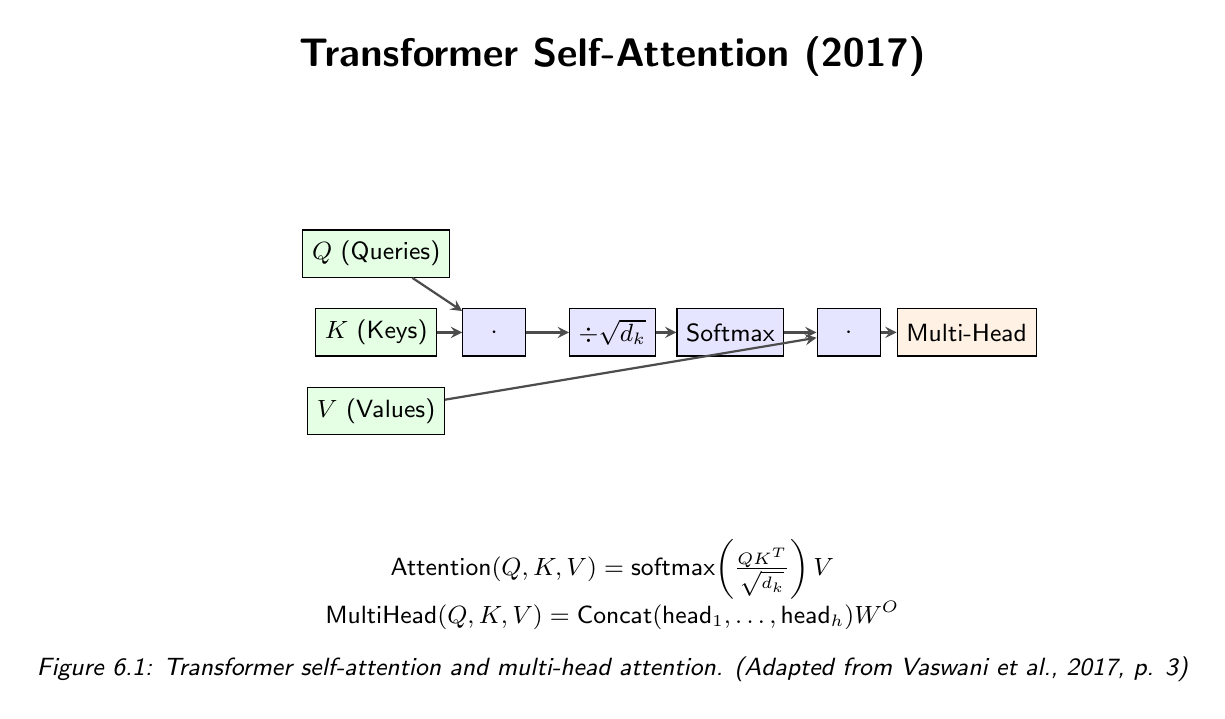
\begin{tikzpicture}[
    block/.style={draw, rectangle, minimum width=0.8cm, minimum height=0.6cm, fill=blue!10, font=\sffamily\small},
    edge/.style={-stealth, thick, draw=black!70},
    label/.style={font=\sffamily\small},
    title/.style={font=\sffamily\Large\bfseries},
    caption/.style={font=\sffamily\small\itshape},
]

\node[title] at (0, 3.5) {Transformer Self-Attention (2017)};

% Inputs
\node[block, fill=green!10] (q) at (-3, 1) {$Q$ (Queries)};
\node[block, fill=green!10] (k) at (-3, 0) {$K$ (Keys)};
\node[block, fill=green!10] (v) at (-3, -1) {$V$ (Values)};

% Scaled dot-product
\node[block] (matmul1) at (-1.5, 0) {$\cdot$};
\node[block] (scale) at (0, 0) {$\div \sqrt{d_k}$};
\node[block] (softmax) at (1.5, 0) {Softmax};

% Output
\node[block] (matmul2) at (3, 0) {$\cdot$};

% Multi-head
\node[block, fill=orange!10] (multi) at (4.5, 0) {Multi-Head};

\draw[edge] (q) -- (matmul1);
\draw[edge] (k) -- (matmul1);
\draw[edge] (matmul1) -- (scale);
\draw[edge] (scale) -- (softmax);
\draw[edge] (softmax) -- (matmul2);
\draw[edge] (v) -- (matmul2);
\draw[edge] (matmul2) -- (multi);

% Equation
\node[align=center, font=\sffamily\small, anchor=north] at (0, -2.5) {
  $\text{Attention}(Q,K,V) = \text{softmax}\!\left(\frac{QK^T}{\sqrt{d_k}}\right)V$ \\
  $\text{MultiHead}(Q,K,V) = \text{Concat}(\text{head}_1, \dots, \text{head}_h)W^O$
};

\node[caption, anchor=north] at (0, -4.0) {
  Figure 6.1: Transformer self-attention and multi-head attention. (Adapted from Vaswani et al., 2017, p. 3)
};

\end{tikzpicture}
\end{document}
